\documentclass[12pt, letterpaper]{../assignment}
\usepackage{graphicx}
\usepackage{courier}
\usepackage{minted}
\usepackage{amsmath}
\usepackage{polynom}
\usepackage{commath}
\usepackage{amssymb}
\usepackage{amsfonts} 
\usepackage{color}
\usepackage{cancel}
\usepackage{enumitem}
\usepackage{graphicx}
\usepackage{multirow}
\usepackage{float}
\usepackage{bm}
\usepackage{tikz}
\usetikzlibrary{shapes,arrows}
\usepackage{booktabs}
\usetikzlibrary{patterns}

% Define Theme Colors
\definecolor{light-gray}{rgb}{0.2,0.2,0.2}
\definecolor{header-blue}{rgb}{0,0,0.7}
% \definecolor{header-blue}{rgb}{0.5137,0.8353,0.9176}
\definecolor{header-blue}{rgb}{0,0.8,0.95}
\definecolor{dark-gray}{rgb}{0.1,0.1,0.1}
\pagecolor{dark-gray}
\color{white}

\usemintedstyle{monokai}
\oddsidemargin = 0pt
\exercisesheet{Module 8}{Midterm Exam}
\student{Austin Barrilleaux}
\university{\color{header-blue}Johns Hopkins University}
\school{\color{header-blue}Whiting School of Engineering}
\courselabel{EN 535.612}
\semester{Fall 2024}
\usepackage[backend=bibtex,style=numeric,sorting=none]{biblatex}
\bibliography{reference}

\definecolor{light-gray}{rgb}{0.2,0.2,0.2}
\setminted{bgcolor=light-gray,frame=lines,rulecolor=white}
\setlength{\parindent}{0pt}

\makeatletter
\patchcmd{\minted@colorbg}{\noindent}{\medskip\noindent}{}{}
\apptocmd{\endminted@colorbg}{\par\medskip}{}{}
\makeatother


\begin{document}

\subsection*{Problem 1}
\subsubsection*{A satellite is in an orbit about the Earth.
The magnitude of the acceleration of this body is $\bm{g(R_e/R)^2}$,
where $\bm{R}$ is the distance from the body to  the center of the Earth,
$\bm{R_e = 6370}$ km is the radius of the Earth,
and $\bm{g = 9.807}\ \textbf{m}/\textbf{s}^2$.
At the position shown, the speed of the body is $\bm{v = 27\ 000 \textbf{km}/\textbf{h}}$.\\
(a) Determine the rate of change of the speed and the radius of curvature of the orbit at this position.\\
(b) Determine $\bm{\dot{R}}$, $\bm{\ddot{R}}$, $\bm{\dot{\theta}}$, and $\bm{\ddot{\theta}}$ at this position.}

\begin{figure}[H]
    \centering
    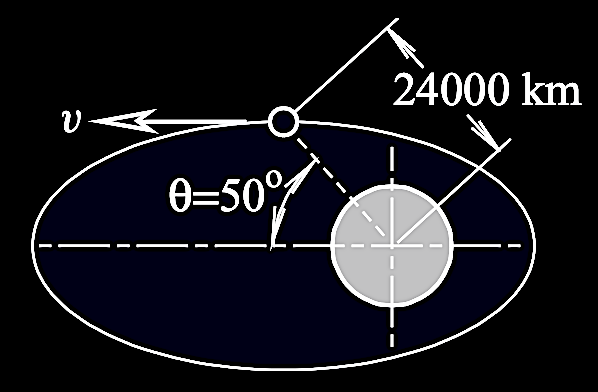
\includegraphics[scale=0.55,frame]{images/Problem_1.png}
\end{figure}

Sketching the following block diagram where, by inspection,
the unit tangent vector $e_t$ is parallel with the velocity vector,
and the normal direction unit vector $e_n$ extends toward the center of curvature
(which is toward the center of the elliptical orbit.)


\begin{center}

    \tikzset{every picture/.style={line width=0.75pt}} %set default line width to 0.75pt        

    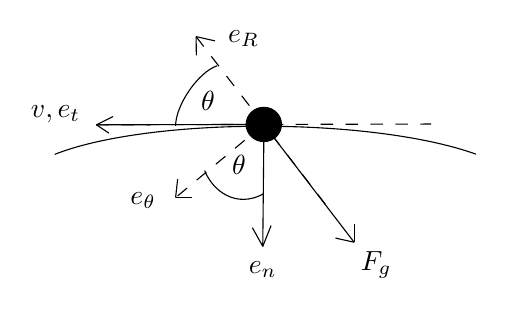
\begin{tikzpicture}[x=0.75pt,y=0.75pt,yscale=-1,xscale=1]
    %uncomment if require: \path (0,235); %set diagram left start at 0, and has height of 235
    
    %Shape: Arc [id:dp5609708917361678] 
    \draw  [draw opacity=0] (78.78,70.17) .. controls (99.75,61.78) and (138.28,56.32) .. (182.31,56.63) .. controls (223.72,56.92) and (260.21,62.24) .. (281.74,70.1) -- (182.11,85.65) -- cycle ; \draw   (78.78,70.17) .. controls (99.75,61.78) and (138.28,56.32) .. (182.31,56.63) .. controls (223.72,56.92) and (260.21,62.24) .. (281.74,70.1) ;  
    %Straight Lines [id:da5753428027341958] 
    \draw    (98.88,55.94) -- (179.5,55.75) ;
    %Flowchart: Connector [id:dp6687027633584581] 
    \draw  [fill={rgb, 255:red, 0; green, 0; blue, 0 }  ,fill opacity=1 ] (171,55.75) .. controls (171,51.19) and (174.81,47.5) .. (179.5,47.5) .. controls (184.19,47.5) and (188,51.19) .. (188,55.75) .. controls (188,60.31) and (184.19,64) .. (179.5,64) .. controls (174.81,64) and (171,60.31) .. (171,55.75) -- cycle ;
    %Straight Lines [id:da46457095104622814] 
    \draw    (179,114.5) -- (179.5,64) ;
    %Straight Lines [id:da07390647343570356] 
    \draw    (223,112.5) -- (179.5,55.75) ;
    %Straight Lines [id:da7232134312062481] 
    \draw  [dash pattern={on 4.5pt off 4.5pt}]  (146.88,13.44) -- (212.13,98.06) ;
    %Straight Lines [id:da15646105402572963] 
    \draw    (98.88,55.94) -- (106.88,51.94) ;
    %Straight Lines [id:da09244139347199365] 
    \draw    (104.88,59.94) -- (98.88,55.94) ;
    %Straight Lines [id:da006527953719763557] 
    \draw    (174,105.5) -- (179,114.5) ;
    %Straight Lines [id:da504994600380142] 
    \draw    (179,114.5) -- (183,104.5) ;
    %Straight Lines [id:da019968065751189146] 
    \draw    (214,110.5) -- (223,112.5) ;
    %Straight Lines [id:da7293082455780622] 
    \draw    (223,103.5) -- (223,112.5) ;
    %Curve Lines [id:da5442907492375646] 
    \draw    (137,56.5) .. controls (137,46.38) and (148,30.5) .. (157,27.5) ;
    %Straight Lines [id:da9878841341299782] 
    \draw    (147,22.5) -- (146.88,13.44) ;
    %Straight Lines [id:da49273640195015456] 
    \draw    (156,15.5) -- (146.88,13.44) ;
    %Straight Lines [id:da8219412910683288] 
    \draw  [dash pattern={on 4.5pt off 4.5pt}]  (98.88,55.94) -- (260.13,55.56) ;
    %Straight Lines [id:da6180368985701121] 
    \draw  [dash pattern={on 4.5pt off 4.5pt}]  (179.5,55.75) -- (137,91) ;
    %Straight Lines [id:da7552791067737405] 
    \draw    (137,91) -- (138,82) ;
    %Straight Lines [id:da9150337620515048] 
    \draw    (145,91) -- (137,91) ;
    %Curve Lines [id:da7268486900699349] 
    \draw    (179.25,89.25) .. controls (166.25,96.25) and (155,88) .. (151,78) ;
    
    % Text Node
    \draw (66,45.4) node [anchor=north west][inner sep=0.75pt]    {$v,e_{t}$};
    % Text Node
    \draw (171,120.4) node [anchor=north west][inner sep=0.75pt]    {$e_{n}$};
    % Text Node
    \draw (225,115.9) node [anchor=north west][inner sep=0.75pt]    {$F_{g}$};
    % Text Node
    \draw (148,38.4) node [anchor=north west][inner sep=0.75pt]    {$\theta $};
    % Text Node
    \draw (161,9.4) node [anchor=north west][inner sep=0.75pt]    {$e_{R}$};
    % Text Node
    \draw (163,69.4) node [anchor=north west][inner sep=0.75pt]    {$\theta $};
    % Text Node
    \draw (114,87.4) node [anchor=north west][inner sep=0.75pt]    {$e_{\theta }$};
    
    
    \end{tikzpicture}
    
\end{center}

From this, we can define the unit tangent vector as: %and the normal direction unit vector as:

$$ \bar{e}_t = \left[\begin{array}{rr} \cos\left(\theta \right) & -\sin\left(\theta \right)\\ \sin\left(\theta \right) & \cos\left(\theta \right) \end{array}\right]
\left[\begin{array}{rr} 1\\ 0 \end{array}\right] = 
\left[\begin{array}{c} \cos\left(\theta \right) \ \bar{e}_R \\ \sin\left(\theta \right) \ \bar{e}_\theta \end{array}\right]  $$

Because $\dot{v}$ is the tangential component of acceleration, we find that:

$$ \dot{v} = \bar{a} \cdot \bar{e}_t = g\left(\frac{R_e}{R}\right)^2
\left[\begin{array}{rr} -1 \ \bar{e}_R \\ 0 \ \bar{e}_\theta \end{array}\right]\cdot
\left[\begin{array}{c} \cos\left(\theta \right) \ \bar{e}_R \\ \sin\left(\theta \right) \ \bar{e}_\theta \end{array}\right]
= -9.807\left(\frac{6370 \times 10^3}{24000 \times 10^3}\right)^2 \cos\left(\theta \right)  $$

This evaluates to:

\begin{answer}
$$ \dot{v} = -0.4441 \ \textbf{m}/\textbf{s}^2  $$
\end{answer}

Looking at the equation for acceleration:

$$ \bar{a} = \dot{v} \bar{e}_t + \frac{v^2}{\rho}\bar{e}_n $$

To solve for the radius of curvature:

$$ \frac{v^2}{\rho}\bar{e}_n = \bar{a} -\dot{v} \bar{e}_t \ \rightarrow
\ \rho = \frac{v^2}{|\bar{a} -\dot{v} \bar{e}_t|} $$

The radius of curvature is:

$$ \rho = \frac{v^2}{|\bar{a} -\dot{v} \bar{e}_t|} =
\frac{\left(27\ 000 \times 10^3/3600\right)^2}{\left|-9.807\left(\frac{6370 \times 10^3}{24000 \times 10^3}\right)^2
\left[\begin{array}{rr} -1\ \bar{e}_R\\ 0 \ \bar{e}_\theta \end{array}\right] -\left(-0.4441\right) 
\left[\begin{array}{c} \cos\left(\theta \right) \ \bar{e}_R \\ \sin\left(\theta \right)\ \bar{e}_\theta \end{array}\right]\right|}
$$

This evaluates to:

\begin{answer}
$$ \rho = 1.0629 \times 10^8 \ \textbf{m}  $$
\end{answer}


Using the following velocity equation:

$$ \bar{v} = \dot{R}\ \bar{e}_R + R \dot{\theta}\ \bar{e}_\theta $$

Looking at the sketch:

$$ \bar{v} = \left(\frac{27\ 000 \times 10^3}{3600}\right)
\left[\begin{array}{c} \cos\left(\theta \right) \ \bar{e}_R \\ \sin\left(\theta \right)\ \bar{e}_\theta \end{array}\right]$$

From these two equations we get that:

\begin{answer}
\begin{equation*}
    \begin{aligned}
        \dot{R} &= \left(\frac{27\ 000 \times 10^3}{3600}\right)\cos\left(\theta \right)
        = 4820.9  \ \textbf{m}/\textbf{s}\\
        \dot{\theta}& = \left(\frac{27\ 000 \times 10^3}{3600}\right)\sin\left(\theta \right)/R
        = 0.0002393  \ \textbf{rad}/\textbf{s}
    \end{aligned}
\end{equation*}
\end{answer}

Using the following acceleration equation:

$$ \bar{a} = \left( \ddot{R} - R \dot{\theta}^2 \right)\bar{e}_R +
\left( R\ddot{\theta} + 2\dot{R}\dot{\theta} \right)\bar{e}_\theta$$

Where:

$$ \bar{a} = -9.807\left(\frac{6370 \times 10^3}{24000 \times 10^3}\right)^2
\left[\begin{array}{rr} -1\ \bar{e}_R\\ 0 \ \bar{e}_\theta \end{array}\right] $$

We get that:

\begin{answer}
\begin{equation*}
    \begin{aligned}
        \ddot{R} &= \bar{a} \cdot \bar{e}_R + R \dot{\theta}^2
        = 0.6845  \ \textbf{m}/\textbf{s}^2\\
        \ddot{\theta}& = \left( \cancelto{0}{\bar{a} \cdot \bar{e}_\theta} - 2\dot{R}\dot{\theta} \right)/R = 
        -9.617\times 10^8 \ \textbf{rad}/\textbf{s}^2
    \end{aligned}
\end{equation*}
\end{answer}

\subsection*{Problem 2}
\subsubsection*{The disk spins about its axis C D at 1200 rev/min as the system rotates about the vertical axis at 20 rev/min.
Both rates are constant.
The angle of elevation of the arm supporting the disk is such that $\bm{\dot{\beta} = 10}$ rad/s and $\bm{\ddot{\beta} = -500}\ \textbf{rad/s}^2$  when $\bm{\beta = 36.87^\circ}$.
Determine the velocity and acceleration of point E,
which is the lowest point on the perimeter of the disk.
Note: the solution for velocity in the text is for a clockwise rotation about the vertical axis}

\begin{figure}[H]
    \centering
    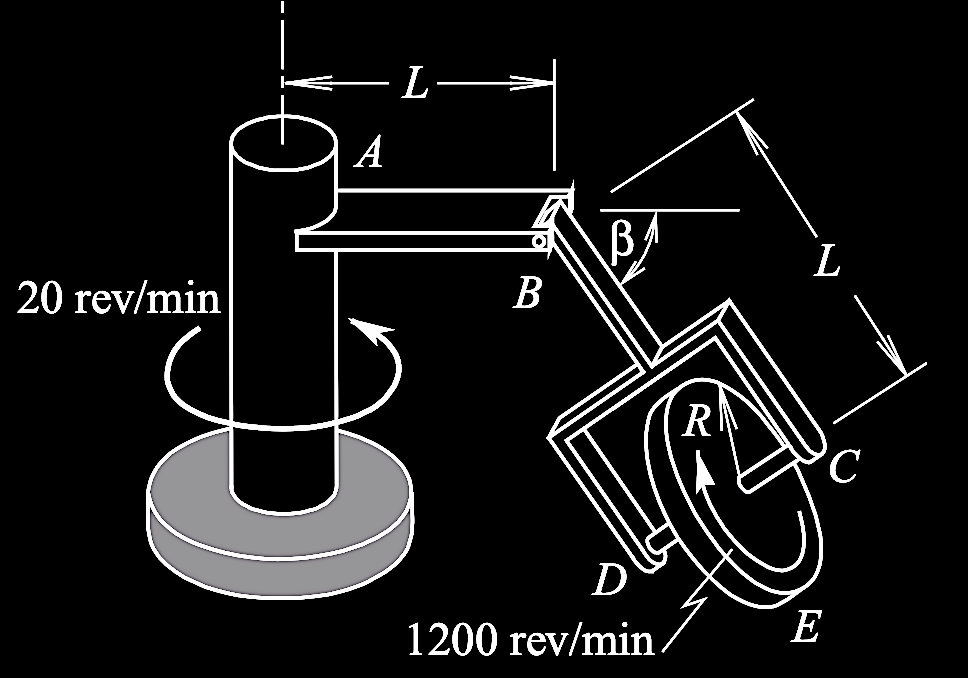
\includegraphics[scale=0.5,frame]{images/Problem_2.png}
\end{figure}

We will solve this problem consistent with the note in the prompt.
\\\\
We will define the following coordinate frames for the system:

\begin{centering}


    \tikzset{every picture/.style={line width=0.75pt}} %set default line width to 0.75pt        

    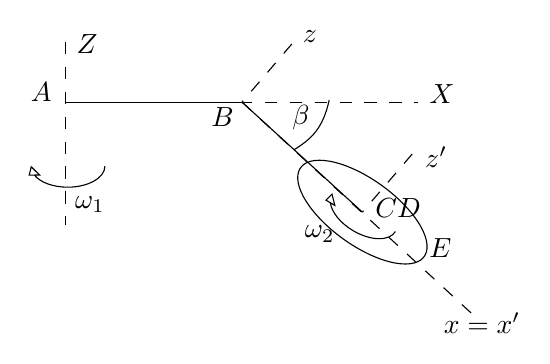
\begin{tikzpicture}[x=0.75pt,y=0.75pt,yscale=-1,xscale=1]
    %uncomment if require: \path (0,182); %set diagram left start at 0, and has height of 182
    
    %Straight Lines [id:da30022602593809844] 
    \draw    (62,54) -- (147,54) ;
    %Straight Lines [id:da8288788542415915] 
    \draw    (147,54) -- (205,107) ;
    %Flowchart: Connector [id:dp18393682558043611] 
    \draw   (181.71,107) .. controls (170.27,93.19) and (171.43,82) .. (184.29,82) .. controls (197.15,82) and (216.85,93.19) .. (228.29,107) .. controls (239.73,120.81) and (238.57,132) .. (225.71,132) .. controls (212.85,132) and (193.15,120.81) .. (181.71,107) -- cycle ;
    %Straight Lines [id:da08328645583785521] 
    \draw  [dash pattern={on 4.5pt off 4.5pt}]  (62,54) -- (232,54) ;
    %Curve Lines [id:da0493598542143765] 
    \draw    (189,53) .. controls (186,67) and (180,72) .. (172,77) ;
    %Straight Lines [id:da10927227437478448] 
    \draw  [dash pattern={on 4.5pt off 4.5pt}]  (62,25) -- (62,113) ;
    %Straight Lines [id:da9966612794201675] 
    \draw  [dash pattern={on 4.5pt off 4.5pt}]  (171,26) -- (147,54) ;
    %Straight Lines [id:da14869123950977747] 
    \draw  [dash pattern={on 4.5pt off 4.5pt}]  (147,54) -- (260,158) ;
    %Straight Lines [id:da3432297912367157] 
    \draw  [dash pattern={on 4.5pt off 4.5pt}]  (229,79) -- (205,107) ;
    %Curve Right Arrow [id:dp22372090927053256] 
    \draw  [fill={rgb, 255:red, 255; green, 255; blue, 255 }  ,fill opacity=1 ] (63.3,94.99) .. controls (73.1,94.9) and (81,90.35) .. (80.95,84.82) -- (80.95,84.82) .. controls (81,90.35) and (73.1,94.9) .. (63.3,94.99) -- cycle ;\draw  [fill={rgb, 255:red, 255; green, 255; blue, 255 }  ,fill opacity=1 ] (63.3,94.99) .. controls (56.02,95.06) and (49.74,92.65) .. (46.97,89.14) -- (49.47,89.12) -- (45.45,85.15) -- (44.47,89.16) -- (46.97,89.14) .. controls (49.74,92.65) and (56.02,95.06) .. (63.3,94.99) -- cycle ;
    %Curve Right Arrow [id:dp9745312713561716] 
    \draw  [fill={rgb, 255:red, 255; green, 255; blue, 255 }  ,fill opacity=1 ] (200.53,115.94) .. controls (208.97,120.93) and (218.09,121.11) .. (220.9,116.36) -- (220.9,116.36) .. controls (218.09,121.11) and (208.97,120.93) .. (200.53,115.94) -- cycle ;\draw  [fill={rgb, 255:red, 255; green, 255; blue, 255 }  ,fill opacity=1 ] (200.53,115.94) .. controls (194.27,112.24) and (190.14,106.93) .. (189.57,102.5) -- (191.73,103.77) -- (190.34,98.3) -- (187.42,101.23) -- (189.57,102.5) .. controls (190.14,106.93) and (194.27,112.24) .. (200.53,115.94) -- cycle ;
    
    % Text Node
    \draw (170,54.4) node [anchor=north west][inner sep=0.75pt]    {$\beta $};
    % Text Node
    \draw (66,20.4) node [anchor=north west][inner sep=0.75pt]    {$Z$};
    % Text Node
    \draw (175,18.4) node [anchor=north west][inner sep=0.75pt]    {$z$};
    % Text Node
    \draw (234,74.4) node [anchor=north west][inner sep=0.75pt]    {$z'$};
    % Text Node
    \draw (243,154.4) node [anchor=north west][inner sep=0.75pt]    {$x=x'$};
    % Text Node
    \draw (236,44.4) node [anchor=north west][inner sep=0.75pt]    {$X$};
    % Text Node
    \draw (65.3,98.39) node [anchor=north west][inner sep=0.75pt]    {$\omega _{1}$};
    % Text Node
    \draw (176,112.4) node [anchor=north west][inner sep=0.75pt]    {$\omega _{2}$};
    % Text Node
    \draw (44,43.4) node [anchor=north west][inner sep=0.75pt]    {$A$};
    % Text Node
    \draw (131,55.4) node [anchor=north west][inner sep=0.75pt]    {$B$};
    % Text Node
    \draw (210,99.4) node [anchor=north west][inner sep=0.75pt]    {$CD$};
    % Text Node
    \draw (236,118.4) node [anchor=north west][inner sep=0.75pt]    {$E$};
    
    
    \end{tikzpicture}
    
\end{centering}

You will note that the \{xyz\} frame and \{x'y'z'\} frame are identical for this problem,
so I will use \{xyz\} to express the coordinate frame at both points from this point.

Constructing the angular velocity vector $\bar{\omega}$ of $\left\{xyz\right\}$ by vectorially adding the simple rotation rates according to:

$$ \bar{\omega} = \omega_1 \bar{e}_1 + \omega_2 \bar{e}_2  + \omega_3 \bar{e}_3$$

This gives us:

$$ \bar{\omega} = -\omega_1 K+ \dot{\beta} j - \omega_2 k$$

Using the following coordinate transformation:

$$ R_\text{rot} = 
\left[\begin{array}{ccc} \cos\left(\beta \right) & 0 & -\sin\left(\beta \right)\\ 0 & 1 & 0\\ \sin\left(\beta \right) & 0 & \cos\left(\beta \right) \end{array}\right]
$$

$$ K = R_\text{rot}
\left[\begin{array}{ccc} 0 \ I \\ 0 \ J \\1 \ K \end{array}\right] = 
\left[\begin{array}{r} -\sin\left(\beta \right) \ i\\ 0 \ j\\ \cos\left(\beta \right) \ k \end{array}\right]
= -\sin\left(\beta \right) i + \cos\left(\beta \right) k$$

This gives us the angular velocity vector in the form:

$$ \bar{\omega} = \left[\begin{array}{r} \omega _{1}\,\sin\left(\beta \right) \ i \\ \dot{\beta } \ j \\ -\omega _{2}-\omega _{1}\,\cos\left(\beta \right) \ k  \end{array}\right] $$

For the angular rotations, the angular velocity is:

\begin{equation*}
\begin{aligned}
\Omega_1 &= -\omega_1 K= \left[\begin{array}{r} \omega _{1}\,\sin\left(\beta \right) \ i \\ 0 \ j \\ -\omega _{1}\,\cos\left(\beta \right) \ k  \end{array}\right]\\
\Omega_2 &= -\omega_1 K+ \dot{\beta} j = \left[\begin{array}{r} \omega _{1}\,\sin\left(\beta \right) \ i \\ \dot{\beta } \ j \\ -\omega _{1}\,\cos\left(\beta \right) \ k  \end{array}\right]\\
\Omega_3 &= \bar{\omega}
\end{aligned}
\end{equation*}

Using the following relative positions:

\begin{equation*}
    \begin{aligned}
        r_{B/A} &= L\left(\begin{array}{c} \cos\left(\beta \right)\ i\\ 0 \ j\\ \sin\left(\beta \right) \ k \end{array}\right)\\
        r_{CD/B} &= L\ i\\
        r_{E/CD} &= R\ i\\
    \end{aligned}
\end{equation*}
    
Solving for velocities along the system from A to E:

\begin{equation*}
    \begin{aligned}
        v_B &= \Omega_1 \times r_{B/A} = \left[\begin{array}{c} 0\\ -2.0944\,L\\ 0 \end{array}\right] \\
        v_{CD} &= v_B + \Omega_2 \times r_{CD/B} = \left[\begin{array}{c} 0\\ -3.7699\,L\\ -10\,L \end{array}\right] \\
        v_E &= v_{CD} + \Omega_3 \times r_{E/CD} = \left[\begin{array}{c} 0\\ -3.7699\,L-127.34\,R\\ -10\,L-10\,R \end{array}\right]
    \end{aligned}
\end{equation*}

Therefore:

\begin{answer}
$$ v_E =   -\left(3.7699\,L+127.34\,R\right) j - 10\left(L+R \right)k $$
\end{answer}

We can solve for the angular rotation at the rotation points using the equation for angular acceleration:

$$ \bar{\alpha} =
\sum_n \left( \dot{\omega}_n \bar{e}_n + \bar{\Omega}_n \times \omega_n \bar{e}_n \right) $$

The relative angular accelerations across the system for points A to E are:

\begin{equation*}
\begin{aligned}
\alpha_1 &= \Omega_1 \times \Omega_1 = 0\\
\alpha_2 &= \alpha_1 + \ddot{\beta} j + \Omega_2 \times \dot{\beta} j\\
\alpha_3 &= \alpha_2 + \Omega_3 \times \omega_2(-k) = \bar{\alpha} % alpha_bar
\end{aligned}
\end{equation*}

Using the acceleration equation:

$$ \bar{a}_P = \bar{a}_O + \bar{\alpha} \times \bar{r}_{P/O} + \bar{\omega} \times \left( \bar{\omega} \times \bar{r}_{P/O} \right)$$

Solving for the acceleration across the system for points A to E:

\begin{equation*}
    \begin{aligned}
        a_B &= 0 + \alpha_1 \times r_{B/A} + \Omega_1 \times \left(\Omega_1 \times r_{B/A}\right)
        =\left[\begin{array}{c} -3.5092\,L\\ 0\\ -2.6319\,L \end{array}\right]\\
        a_{CD} &= a_B + \alpha_2 \times r_{CD/B} + \Omega_2 \times \left(\Omega_2 \times r_{CD/B}\right)
        =\left[\begin{array}{c} -106.32\,L\\ 25.133\,L\\ 495.26\,L \end{array}\right]\\
        a_E &= a_{CD} + \alpha_3 \times r_{E/CD} + \Omega_3 \times \left(\Omega_3 \times r_{E/CD}\right)
        =\left[\begin{array}{c} -106.32\,L-16315\,R\\ 25.133\,L+25.133\,R\\ 495.26\,L+182.07\,R \end{array}\right]
    \end{aligned}
\end{equation*}

Therefore:

\begin{answer}
$$ a_E = -(106.32\,L+16315\,R)\ i + 25.133(L+R)\ j + (495.26\,L+182.07\,R)\ k $$
\end{answer}

These solutions match the text.


% We can compute the velocity vector as:

% $$ \bar{v} = \left( \frac{27\ 000\ \times 10^3}{3600} \ \text{m}/\text{s} \right) $$


% % \color{white}
% \hspace*{6em}\inputminted[frame=leftline,fontsize=\footnotesize]{matlab}
% {./matlab/Q6_8.m}
% % \color{black} 

% \begin{figure}[H]
%     \centering
%     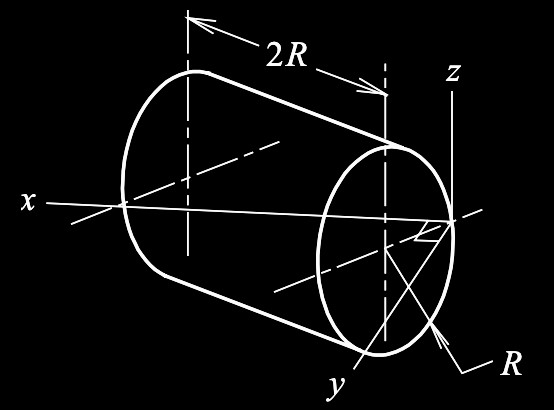
\includegraphics[scale=0.7,frame]{images/Q5_13.png}
% \end{figure}




\end{document}

